%\documentclass[handout]{beamer}
\documentclass{beamer}
 
\usetheme[numbering = fraction, progressbar = none, background = light, sectionpage = progressbar]{metropolis}
\usepackage{amsmath}
\usepackage{synttree}
\usepackage{tabu}
\usepackage{graphicx}
\usepackage{setspace}

\title{Econ 103 -- Statistics for Economists}
\subtitle{Chapter 3: Group Work}
\author{Mallick Hossain}
\date{}
\institute{University of Pennsylvania}
\begin{document} 

%%%%%%%%%%%%%%%%%%%%%%%%%%%%%%%%%%%%%%%%
\begin{frame}
	\titlepage 
\end{frame} 

\section{Dice}
%%%%%%%%%%%%%%%%%%%%%%%%%%%%%%%%%%%%%%%%
\begin{frame}
\frametitle{``Odd Question'' \# 4}
    To throw a total of 7 with a pair of dice, you have to get a 1 and a 6, or a 2 and a 5, or a 3 and a 4.
    To throw a total of 6 with a pair of dice, you have to get a 1 and a 5, or a 2 and a 4, or a 3 and 
    another 3.
	\vspace{1em}
	With two fair dice, you would expect:
	\begin{enumerate}[(a)]
		\item To throw 7 more frequently than 6.
		\item To throw six more frequently than 7.
		\item To throw 6 and 7 equally often.
	\end{enumerate}
\end{frame}

\section{Coin Flipping}
%%%%%%%%%%%%%%%%%%%%%%%%%%%%%%%%%%%%%%%
\begin{frame}
\frametitle{``Odd Question'' \# 5}
	``Imitate'' a coin. That is, write down a sequence of 100 H (for heads) and T (for tails) without                                                                                                                     
	tossing a coin--but a sequence that you think will fool everyone into thinking it is the reporting of 
	tossing a fair coin.		
\end{frame}

%%%%%%%%%%%%%%%%%%%%%%%%%%%%%%%%%%%%%%%%
\begin{frame}
\frametitle{Which of these is a real sequence of coin flips?}
	\small
	\begin{block}{Exhibit A}
	H H H H T H H T T T H H T T T H T T T H T T H H T \\
	T T T H T T T H T H T T H H H H T T T T T H H H H \\
	H T T H T T H H T T H H H H H T H H T H T H T H T \\
	T H H T H H T T T H T T T T T T T T T H H T T T T 
	\end{block}
	
	\begin{block}{Exhibit B}
	H H T H T T T H H T H H H T H T T T H T H H T T T\\
	T H H T T T H H H T H T T T H T T H H T H H T H T\\
	T T H H H T H T T H T H H T	T H H H T H T T H H H\\
	T T H H H H T H T T H H T T T H H T H H H T T H T
	\end{block}
\end{frame}

%%%%%%%%%%%%%%%%%%%%%%%%%%%%%%%%%%%%%%%%
\begin{frame}
\frametitle{How could we tell which are the real coin flips?}
    \begin{quote}
	Hardly anyone making up a sequence of 10 tosses puts in a run of 7 heads in a row. It is true that 
	the chance of getting 7 heads in a row with a fair coin is only 1/64. But in tossing a coin 100 times, 
	you have at least 93 chances to start tossing 7 heads in a row, because \alert{each of the first 93 
	tosses could begin a run of 7.} It is more probable than not, in 100 tosses, that you will get 7 
	heads in a row. It is certainly more probable than not, that you will get at least 6 heads in a row. 
	Yet almost no one writes down a pretend sequence, in which there are even 6 heads in a row.
	\end{quote}
\end{frame}

%%%%%%%%%%%%%%%%%%%%%%%%%%%%%%%%%%%%%%%%
%Some macros for the Venn Diagrams
\def\eventA{(-0.35,0) circle (1.2)}
\def\eventB{(1.35,0) circle (1.2)}
\def\samplespace{(-2,-2) rectangle (3,2)}
%%%%%%%%%%%%%%%%%%%%%%%%%%%%%%%%%%%%%%%%
%Some macros for collectively exhaustive and mutually exclusive sets
\def\Srect{(-2,-2) rectangle (4,2)}
\def\Arect{(-2,-2) rectangle (0,2)}
\def\Brect{(0,-2) rectangle (2,2)}
\def\Crect{(0,2) rectangle (4,2)}
\def\Devent{(1.6,-0.3) circle (1.3)}
\def\Eevent{(-1,1.2) circle (0.5)}
%%%%%%%%%%%%%%%%%%%%%%%%%%%%%%%%%%%%%%%%
%Some macros for the Venn Diagrams
\def\EventA{(-0.35,0) circle (1.2)}
\def\EventB{(1.35,0) circle (1.2)}
\def\EventC{(-0.35,0) circle (0.6)}
\def\EventD{(0,0) circle (1.6)}
\def\SampleSpace{(-2,-2) rectangle (3,2)}

\section{Cards}
%%%%%%%%%%%%%%%%%%%%%%%%%%%%%%%%%%%%%%%%

\begin{frame}

\frametitle{Poker -- Deal 5 Cards, Order Doesn't Matter}

\begin{block}{Basic Outcomes}
\vspace{0.3em} 
$\displaystyle{52 \choose 5}$ possible hands
\end{block}
\begin{block}{How Many Hands have Four Aces? } \pause
\alert{48 (\# of ways to choose the single card that is not an ace)}
\end{block}

\begin{block}{Probability of Getting Four Aces}
\vspace{0.3em} 
$48/\displaystyle{52 \choose 5} \approx 0.00002$
\end{block}


\end{frame}
%%%%%%%%%%%%%%%%%%%%%%%%%%%%%%%%%%%%%%%%
\begin{frame}
\frametitle{Poker -- Deal 5 Cards, Order Doesn't Matter}
\begin{block}{What is the probability of getting 4 of a kind?}
	\only<2->{\begin{itemize}
		\item 13 ways to choose \emph{which} card we have four of
		\item 48 ways to choose the last card in the hand 
		\item $13 \times 48 = \alert{624}$ 
	\end{itemize}}
\end{block}
\vspace{0.3em} 
\only<2->{$624/\displaystyle{52 \choose 5} \approx 0.00024$}

\end{frame}

\section{Tennis Tournament}
%%%%%%%%%%%%%%%%%%%%%%%%%%%%%%%%%%%%%%%%
\begin{frame}
\frametitle{A Fairly Ridiculous Example}

Roger Federer and Novak Djokovic have agreed to play in a tennis tournament against six Penn professors. Each player in the tournament is randomly allocated to one of the eight rungs in the ladder (next slide). Federer always beats Djokovic and, naturally, either of the two pros always beats any of the professors. What is the probability that Djokovic gets second place in the tournament? 



\end{frame}
%%%%%%%%%%%%%%%%%%%%%%%%%%%%%%%%%%%%%%%%

\begin{frame}
\begin{figure}
\centering
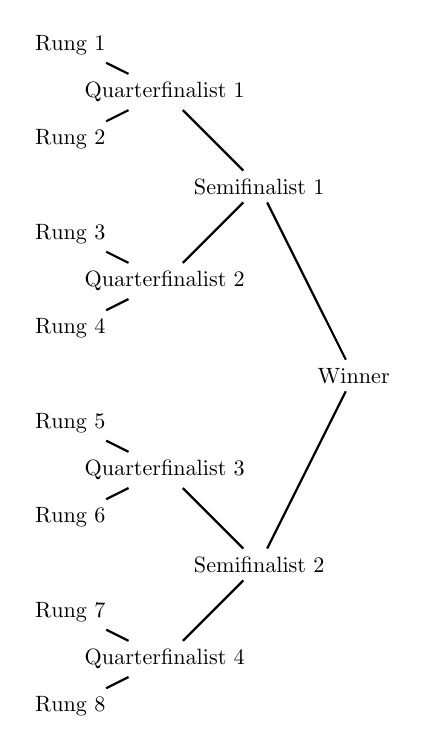
\begin{tikzpicture}[thick,scale=0.8, every node/.style={transform shape},grow'=left]
\node {Winner} 
  [sibling distance=6cm]
  child {node {Semifinalist 2}
  [sibling distance=3cm]
    child {node {Quarterfinalist 4}
    	    [sibling distance=1.5cm]
    	child {node {Rung 8}}
    	child {node {Rung 7}}
    }
    child {node {Quarterfinalist 3}
        [sibling distance=1.5cm]
    	child {node {Rung 6}}
    	child {node {Rung 5}}
    }
  }
  child {node {Semifinalist 1}
  [sibling distance=3cm]
    child {node {Quarterfinalist 2}
    [sibling distance=1.5cm]
    	child {node {Rung 4}}
    	child {node {Rung 3}}
    }
    child {node {Quarterfinalist 1}
        [sibling distance=1.5cm]
    	child {node {Rung 2}}
    	child {node {Rung 1}}
    }
  };
\end{tikzpicture}
\raisebox{4.4em}{\includegraphics[scale=0.8]{./images/tennisplayers}} 
\end{figure}


\end{frame}

%%%%%%%%%%%%%%%%%%%%%%%%%%%%%%%%%%%%%%%%
\begin{frame}
  \frametitle{Solution: Order Matters!}
  \begin{block}{Denominator}
	$8!$ basic outcomes -- ways to arrange players on tournament ladder.
  \end{block}
  \begin{block}{Numerator}
   Sequence of three decisions:
   \begin{enumerate}
    \item Which rung to put Federer on? (8 possibilities)
    \item Which rung to put Djokovic on? 
      \begin{itemize}
        \item For any given rung that Federer is on, only 4 rungs prevent Djokovic from meeting him until the final.
      \end{itemize}
    \item How to arrange the professors? ($6!$ ways)
   \end{enumerate}
  \end{block}
\alert{$$\frac{8 \times 4 \times 6!}{8!} = \frac{8\times 4}{7\times 8} = 4/7 \approx 0.57$$}

\end{frame}

\section{The Card Game}
%%%%%%%%%%%%%%%%%%%%%%%%%%%%%%%%%%%%%%%%
\begin{frame}
\frametitle{Three Cards, Each with a Face on the Front and Back}
\begin{figure}
\fbox{\includegraphics[scale = 0.75]{./images/gaga}}
\hspace{1em}
\fbox{\includegraphics[scale = 0.75]{./images/obama}}
\end{figure}
\begin{enumerate}
	\item Gaga/Gaga
	\item Obama/Gaga
	\item Obama/Obama
\end{enumerate} 
\begin{alertblock}{I draw a card at random and look at one side: it's Obama. What is the probability that the other side is also Obama?\\\hfill}\end{alertblock}
\end{frame}

%%%%%%%%%%%%%%%%%%%%%%%%%%%%%%%%%%%%%%%%
\begin{frame}

% Set the overall layout of the tree
\tikzstyle{level 1}=[level distance=3.5cm, sibling distance=3.5cm]
\tikzstyle{level 2}=[level distance=3.5cm, sibling distance=2cm]

% Define styles for bags and leafs
\tikzstyle{bag} = [text width=4em, text centered]
\tikzstyle{end} = [circle, minimum width=3pt,fill, inner sep=0pt]


\begin{tikzpicture}[thick,scale=0.94, every node/.style={transform shape},grow=right]
\node[bag]{Choose Card}
    child {
        node[bag] {Obama Obama}        
        child {
                node[end, label=right:
                    {Obama}] {}
                edge from parent
                node[below]  {$\frac{1}{2}$}
            }
            child {
                node[end, label=right:
                    {Obama}] {}
                edge from parent
                node[above] {$\frac{1}{2}$}
            }
            edge from parent 
            node[below]  {$\frac{1}{3}$}
    }
        child {
        node[bag] {Obama Gaga}        
        child {
                node[end, label=right:
                    {Gaga}] {}
                edge from parent
                node[below]  {$\frac{1}{2}$}
            }
            child {
                node[end, label=right:
                    {Obama}] {}
                edge from parent
                node[above] {$\frac{1}{2}$}
            }
            edge from parent 
            node[above]{$\frac{1}{3}$}
    }
    child {
        node[bag] {Gaga Gaga}        
        child {
                node[end, label=right:
                    {Gaga}] {}
                edge from parent
                node[below]  {$\frac{1}{2}$}
            }
            child {
                node[end, label=right:
                    {Gaga}] {}
                edge from parent
                node[above] {$\frac{1}{2}$}
            }
        edge from parent         
            node[above] {$\frac{1}{3}$}
    };
\end{tikzpicture}

\end{frame}

%%%%%%%%%%%%%%%%%%%%%%%%%%%%%%%%%%%%%%%%
\begin{frame}
\frametitle{Actual Interview Question}
\begin{itemize}
	\item Imagine a chess board
	\item You start in the top left corner of the board
	\item Your goal is to get to the bottom right
	\item You can only move down or right
	\item How many possible ways are there to get to the bottom right?
\end{itemize}

\centering
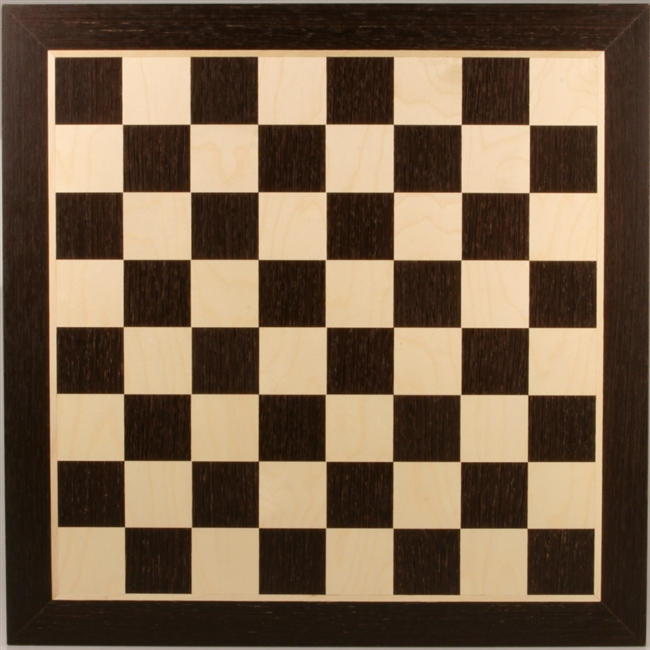
\includegraphics[scale=0.25]{./images/chess.jpg}

\end{frame}

%%%%%%%%%%%%%%%%%%%%%%%%%%%%%%%%%%%%%%%%
\begin{frame}
\frametitle{The Secretary Problem (aka the Marriage Problem)}
\begin{itemize}
	\item You have $n$ applicants for a secretary position
	\item There is a ranking of the candidates (but you cannot observe it)
	\item You can only determine relative ranks (this person was better than that person)
	\item Your goal is to choose the best candidate
	\item You interview them one at a time, but at the end of the interview, you have to either reject them or give them an offer
	\item Once you've rejected someone, you cannot get them back
	\item What strategy will give you the highest chance of success?
\end{itemize}

\end{frame}

%%%%%%%%%%%%%%%%%%%%%%%%%%%%%%%%%%%%%%%%
\begin{frame}
\frametitle{The Secretary Problem (aka the Marriage Problem)}
\begin{itemize}
	\item \textbf{Strategy:} Let some number $k$ candidates go by and then pick the next candidate that is better than anyone you've seen so far.
	\item \textbf{Question:} What should $k - 1$ be?
\end{itemize}

\end{frame}

\end{document}
